\documentclass[14pt, a4paper]{extarticle}
\usepackage[left=2cm,right=2cm,bottom=3cm,top=2cm]{geometry}

\usepackage[utf8]{inputenc}
\usepackage[russian]{babel}
\usepackage{graphicx}
\usepackage{float}
\usepackage{caption}
\usepackage{subcaption}
\usepackage{url}
\usepackage{multirow}
\usepackage{mathtools}
\usepackage{amsmath}
\usepackage{indentfirst}
\usepackage{multirow}
\usepackage{rotating} 
\usepackage{tabu}
\usepackage{cases}

\DeclarePairedDelimiter{\abs}{\lvert}{\rvert}

\linespread{1.25}

\begin{document}

\section*{Введение}
\addcontentsline{toc}{section}{Введение}

В последнее время всё более актуальной становится проблема навигации внутри помещений, а также предоставления посетителям услуг, основанных на их местоположении и предпочтениях. Здания становятся всё более объёмными и нередко имеют довольно сложную структуру, ориентироваться в которой могут лишь те, кто постоянно посещает такие здания, а для неподготовленного человека ориентирование в таких местах превращается в пытку.

Благодаря indoor-навигации (навигации внутри помещений) появляются новые инструменты для маркетинга: проходя мимо магазина, человек может моментально узнать о проводимых в нем акциях, мероприятиях, товарах и предоставляемых услугах, благодаря всплывающему сообщению на экране своего телефона (так называемом “Geo-fencing”, причём предложенные ему предложения будут учитывать его интересы, так как можно учитывать информацию о его прошлых покупках), либо просто получить уведомление при приближении к определенному месту (второе направление indoor-навигации, называемое «Geo-aware»), а владельцы – получать статистическую информацию («тепловые карты» посетителей – своеобразный и очень мощный offline-аналог Google Analytics), основанные на перемещениях клиентов внутри торговых залов (таким образом понять, какие отделы и товары пользуются повышенным интересом, очень легко). Рынок подобной геоконтекстной рекламы уже измеряется миллиардами долларов, и с развитием систем indoor-навигации ожидается его стремительный рост.

Кроме того, решения, применяемые в indoor-навигации, помогают и в ориентировании вне зданий, на улице – там, где в условиях плотной застройки использование систем спутниковой навигации затруднено. Особенно эта проблема актуальна для Японии с высокой плотностью городской застройки.

Bluetooth-маяки, представляющие собой один из способов решения проблемы локации, также являются частью Интернета вещей, и способны изменить представление о самом Интернете вещей. Google представила концепцию "physical web", которая призвана объединить два мира: реальный и виртуальную Интернет-сеть. Смартфон, сканируя ближайшие к нему маячки, получает из их сигнала встроенные URL-ссылки, доступные пользователю. Таким образом, пользователь может мгновенно получить доступ к информации, определенной в ближайшем локационном контексте. Кроме того, это шаг навстречу унифицированному, бесшовному интерфейсу взаимодействия с цифровым миром.

Но современный этап развития технологии внутренней навигации представлен в основном технологиями для навигации роботов по маякам. Кроме того, существует множество готовых продуктов и платформ от производителей с мировым именем. В то же время сообщество программистов не располагает подходящими материалами, чтобы оценить существующие варианты алгоритмов трилатерации и выбрать лучший способ в рамках собственных приложений или свободно распространяемыми библиотеками, которые можно было бы легко подстроить в рамках решаемой задачи.

Именно это и подтолкнуло меня к решению задач, поставленных в рамках настоящей работы.    \clearpage \newpage
\section{Постановка задачи}

Цель работы:
\begin{enumerate}
    \item
    Проанализировать и сравнить различные методы трилатерации, используемые при решении задачии навигации внутри помещений:
    \begin{enumerate}
        \item
        метод, основанный на поиске области пересечения сфер;
        \item
        метод, основанный на поиске силового центра;
        \item
        продвинутый геометрический алгоритм.
    \end{enumerate}
    \item
    Разработать библиотеку, содержащую реализации вышеперечисленных алгоритмов.
\end{enumerate}

К разрабатываемому проекту выдвинуты следующие требования:
\begin{enumerate}
    \item
    Поддержка различных методов трилатерации;
    \item
    Работа алгоритмов должна быть максимально оптимизирована как по скорости вычислений, так и по объему занимаемой памяти;
    \item
    Библиотека должна легко подключаться в проект при помощи менеджеров управления зависимостей CocoaPods или Carthage;
    \item
    Первоначальная настройка библиотеки в проекте должна содержать минимум кода и быть интуитивно понятной.
\end{enumerate}    \clearpage \newpage
\section{Глоссарий}

LBS (“Location Based Service”) – сервис, основанный на местоположении.

GPS (“Global Positioning System”) – глобальная система позиционирования.

LBA (“Location Based Advertising”) – геоконтекстная реклама.

RFID (“Radio Frequency Identification”) – радиочастотная идентификация.

NFC (“Near Field Communication”) – ближняя бесконтактная связь.

BLE (“Bluetooth Low Energy”) – беспроводная технология Bluetooth с низким энергопотреблением.

SDK (“Standard Developer Kit”) – стандартный набор разработчика.

API (“Application Programming Interface”) – интерфейс программирования приложений.

CMS (“Content Management System”) – система управления содержимым.

REST (“Representational State Transfer”) – передача репрезентативного состояния.

BVH (“Bounding Volumes Hierarchy”) – иерархия ограничивающих объемов.

DoS (“Denial of Service”) – отказ в обслуживании.

AGA (“Advanced Geometric Algorithm”) – продвинутый геометрический алгоритм.

Спуффинг маячков (“beacon spoofing”) – тип хакерской атаки, заключающийся в выставлении поддельного маячка, настроенного с параметрами маяков некоторой существующей группы маяков.

Пиггибэкинг маячков (“beacon piggybacking”) – тип хакерской атаки, основанный на использовании параметров маячков, определенных в одном приложении, в стороннем приложении, принадлежащем третьим лицам. Сам же термин “piggybacking” с английского можно перевести как «несанкционированное проникновение вслед за зарегистрированным пользователем».

Fingerprints (с англ. буквально «отпечатки пальцев») – способ нахождения положения пользователя на основе сравнения ряда измерений расстояний до маяков с набором эталонных измерений, определенных для известных локаций.

Фильтр частиц (“particle filter”) – метод трилатерации, в котором в процессе генерации частицы (точки в двумерном пространстве) все лучше приближают истиное положение пользователя, а наименее значимые исключаются из рассмотрения.   \clearpage \newpage
\section{Анализ задачи}

В случае спутниковой навигации (GPS/Глонасс) существуют сервисы Out\-Door, благодаря которым пользователь может узнать о ближайших кафе, ресторанах, гостиницах и других местах благодаря тому, что известно его текущее местоположение. А благодаря сервисам indoor-навигации возможно без проблем и оперативно найти ближайшую стойку регистрации в здании аэропорта, экспонат в музее, отдел и полку с нужным вам товаром в магазине, свободное место на парковке, и многое другое. 

В качестве наиболее значимых примеров можно перечислить следующие:
\begin{itemize}
    \item
    \textit{Розничная торговля.} Установив маячки, становится возможным приветствовать клиента, сообщать ему о новых поступлениях и предложениях, когда тот находиться рядом, а заодно узнать, как он движется внутри заведения и у каких товаров проводит больше времени, - верный ключ к оптимизации для маркетологов.
    \item
    \textit{Городской туризм.} Оказавшись рядом с объектом достопримечательности, пользователь получает информацию о месте. Этот же механизм поможет туристам получать уведомления о прибытии интересующего их транспорта к указанному месту.
    \item
    \textit{Управление кадрами.} Используя механизм маячков, становится легко следить за тем, сколько времени тратит в офисе каждый из сотрудников, если установить пару датчиков на вход. Также возможно быстро организовывать собрания: достаточно разослать оповещение каждому, кто не находится на рабочем месте.
    \item
    \textit{Фитнес-услуги.} Новички могут получать информацию о предназначении того или иного тренажера, а также инструкцию по его правильному использованию. Кроме того, для любого посетителя может оказаться полезной индивидуальная программа тренировок, которая бы не только замеряла время на подход и перерывы в занятиях, но и указала бы, где найти тренажер, наиболее эффективный для следующего этапа тренировок.
    \item
    \textit{Ресторанный бизнес.} В данной сфере оригинальной идеей будет выделение уникальных посетителей заведения: это не только информирует владельца ресторана, но и позволит разработать систему персональных скидок и условий. К примеру, клиент-завсегдатай может сформировать свой заказ заранее, и, как только он войдет в заведение, заказ автоматически поступит на кухню.
    \item
    \textit{Дом.} Bluetooth-маячки способны расширить функциональность умного дома или заменить многие сенсоры. В способы применения входят, например, умное освещение или блокирование входной двери. В данной сфере развивается, например, команда "airfy Beacon" \cite{web:airfyBeacon}. 
    \item
    \textit{Гостиницы.} Маячок на ресепшне улавливает гостей и сразу позволяет отобразить информацию о постоянных посетителях с их историей пребывания, что в итоге уменьшает время заселения. Такой системой пользуется сервис Mahana \cite{web:crunchTime}.
    \item
    \textit{Концертные площадки и стадионы.} Поклонники музыкантов и спортсменов получают подробную справочную информацию и статистику. Желающие могут приобрести билеты на будущие события. С нового сезона так работает приложение Главной лиги бейсбола США, на основных стадионах которой поставили маячки \cite{web:MLB}. 
    \item
    \textit{Дейтинг.} Маячки в барах улавливают людей с поддерживаемыми приложениями. Если посетители хотят с кем-нибудь познакомиться, то получат уведомление, через которое смогут увидеть профили тех, кто находится поблизости. Функцией уже вовсю пользуются конкуренты Tinder — например, Mingleton \cite{web:Mingleton}.
    \item
    \textit{Школы и университеты.} Преподавателям не нужно отмечать, кто из школьников и студентов ходит на занятия: система сама учитывает всех пришедших и, если необходимо, оповещает родителей. Кроме того, специальное приложение может предлагать учащимся вакансии, делить аудитории, высылая в разные части разный контент. Также в приложении может быть встроенный мессенджер и специальная кнопка для застенчивых студентов, которые стесняются задать вопрос на занятии. Уже есть приложения, которые справляются с некоторыми этими задачами, например, BeHere.
    \item
    \textit{Фестивали и конференции.} Посетителям высылают карту и расписание, справочную информацию о тех, кто выступает, и предлагают подойти к стендам. Крупнейшие площадки уже опробовали технологию: на SXSW с помощью iBeacon устраивали опросы, обсуждения среди участников и помогали разобраться, где что находится, а на кинофестивале «Трайбека» зрители могли сориентироваться, когда и где покажут нужный им фильм. Необычнее же всего технологию использовали на Каннском кинофестивале. Официальное приложение показывало, кто из гостей где находится, а также отображало ссылку на профиль каждого в LinkedIn — так было удобнее налаживать бизнес-контакты.
\end{itemize}

Благодаря большим коммерческим перспективам, направление indoor-на\-ви\-га\-ции становится всё более востребованным и уже привлекло внимание таких крупных игроков на рынке, как Google, Apple, Qualcomm, Broadcom, Sony и другие, и в это, без сомнения, перспективное направление уже инвестируются сотни миллионов долларов %\cite{web:meetBeacons}.

Всемирно известная компания PayPal обозначила свой курс развития, как «инвестиции в мобильные технологии, а также возрождение розничной торговли с помощью, опять же, технологий» %\cite{web:paypal}. 
Разрабатываемое ими устройство – PayPal Beacon – как раз реализованный шаг в данном направлении. Оно представляет собой портативный считыватель дебетовый и кредитных карт, по функциональности не отличающийся от тех, что зачастую установлены на кассах. С помощью него, кроме непосредственно оплаты, возможно и локационное взаимодействие: местоположение пользователя является связующим звеном, помогающим определить, что он находится в конкретном заведении, и мгновенно предложить авторизацию для совершения дальнейших покупок.   \clearpage \newpage
    \subsection{Анализ примеров успешного внедрения}

Международная платежная система MasterCard, Мультимедиа Арт Музей Москва, агентства Digitalizm и Insight ONE объявляют о запуске интерактивного гида <<MasterCard Бесценные города – Твой МАММ>> - первого в России интерактивного гида по музею, разработанного с применением технологии iBeacon. Таким образом проект решает современными инновационными средствами образовательные и маркетинговые задачи в пространстве музея \cite{web:firstMuseum}.

Крупная сеть аптек Rite Aid установила маячки в более чем 4500 торговых точках, воспользовавшись услугами компании inMarket. inMarket знаменит услугами по изготовлению и установке Bluetooth-маячков собственного, защищенного от атак хакеров, формата \cite{web:RiteAid}.

В другом материале InMarket описывает кейс американского производителя продуктов питания Hillshire Brands, который хотел повысить продажи определенного сорта выпускаемых им сосисок. Разработав и внедрив приложение, работающее на основе iBeacon, компания получила увеличение узнаваемости марки сосисок на 36\% и рост общего объема продаж в 10 американских магазинах, где были установлены маячки iBeacon \cite{web:Hillshire}.

Zatarain - первая в мире компания по производству фасованных потребительских товаров, которая внедрила технологию iBeacon. В своих магазинах компания в определенных контрольных точках установила маячки iBeacon. Оказываясь рядом с такими точками, посетители получали push-уведомления, которые мотивировали покупателей искать продукты Zatarain в магазине. Люди сканировали продукты бренда и получали за это призовые очки. Покупатели взаимодействовали с брендированнной мобильной страницей, держа в руках сам продукт от Zatarain. В итоге, люди, которые получали iBeacon-уведомления от компании, в 5 раз чаще использовали ее приложение, что соответственно привело к большому вовлечению потребителей в магазине. Оказалось, что посетители магазина, которые взаимодействовали с продуктом на контрольных точках, в 130 раз охотнее покупали его, чем остальные. Для сравнения -  обычный мобильный баннер увеличивает намерение делать покупки в среднем на 3\% \cite{web:Zatarin}.

Известный продавец обуви Timberland тестировал технологию iBeacon от Swirl в двух своих магазинах в Нью-Йорке и Бостоне. Результаты получились следующими: пользователи мобильного приложения просматривали 72\% рекламных предложений от общего количества приходящих на их смартфоны, а 35\% из них купили рекламируемый товар. Около 750 покупателей получили 20\% скидку от Timberland \cite{web:Timberland}.

“Virgin Atlantic” и аэропорт «Хитроу» тестируют сервис информирования авиапассажиров на основе маяков \cite{web:Heathrow}. В Московском аэропорту «Шереметьево» данная система уже частично в ходу, инженерам потребуется около 7500 устройств, чтобы покрыть площадь в 500 тысяч квадратных метров. Следом за «Шереметьево» к использованию iBeacon-навигации должны подключиться аэропорты «Домодедово» и «Внуково» \cite{web:Aeroports}.

Свидетельством этого является следующий факт: один из крупнейших мировых магазинов "Macy's"  планируют установить в залах своих торговых центров около 4000 таких устройств \cite{web:Macy}. 

В прошлом году на Российском Интернет Форуме <<РИФ+КИБ>> в здании было установлено 200 маячков, и всем посетителям была наглядно продемонстрирована система навигации внутри помещения \cite{web:RifKib}.

\textit{Выводы о внедрении}: 
Компания - производитель маячков Swirl провела исследование, результаты которого показали, что пользователи мобильных приложений, в первую очередь (80\%), желают получать push-уведомления о скидках. По данным того же исследования люди специально будут отключать возможность получения push-уведомлений, если в них не будет полезной информации (то есть тех же акций и скидок) или сообщения будут не релеванты их интересам или месторасположению.

Подтверждают эти выводы и исследования ювелирного магазина Alex\&Ani, внедрившего в свою работу iBeacon технологии. Вот его результаты:
\begin{itemize}
    \item
    93\% опрашиваемых покупателей согласилось с тем, что мобильные рекламные предложения, которые они получают в магазине увеличивают вероятность их покупки.
    \item
    90\% утверждают, что мобильные предложения заставляют их чаще посещать магазин.
    \item
    88\% сказали, что опыт пребывания в магазине становится более интуитивным и легким.
\end{itemize}

Cогласно исследованию Google, 84\% посетителей пользуются мобильными устройствами, находясь в магазинах, причём 50\% проводят в них не менее 15 минут \cite{web:GoogleShopExpirience}.

По данным аналитики, сегодня во время визита в магазин в 2 раза больше покупателей обращается за информацией о товарах и скидках к мобильному приложению, нежели к продавцу-консультанту. Мобильные решения сегодня полностью меняют картину маркетинговой активности потребителей \cite{web:CasesZero}.  
    \subsection{Анализ существующих платформ}

В рамках рассматриваемой работы были проанализированы главные существующие платформы, способные без программирования строить iBeacon-приложения, а также выделены их главные особенности.

\begin{itemize}
    \item
    Indoors (http://indoo.rs/). Компания представляет целую платформу для навигации в помещениях. В перечень инструментов входят инструменты для моделирования пространства, расстановки маяков и их калибровки. С результами работы можно ознакомиться в демонстрационном приложении.
    \item
    LabWerk (http://labwerk.com). Основной продукт данной корпорации - решение для музеев mApp. Как следствие, существует функциональность для создания статей об объектах выставок и экспонатах, а также социальные элементы вроде создания опросов. Предусмотрена и карта заведения, отображающее текущее положение пользователя. Кроме того, система умеет собирать статистику о посещениях.
    \item
    ShopJoy (http://shopjoy.se). Авторы данной платформы предоставляют возможность тонко настраивать push-уведомления для всех клиентов на основе их персонализации. За основу берется информация, указанная пользователем при регистрации.
    \item
    LocalSocial (https://www.mylocalsocial.com). В целом у продукта можно выделить две сильные стороны. Во-первых, это система управления содержимым, через которую легко выделить географические зоны и зарегистрировать в них маячки. Во-вторых, это система лояльности пользователей: возможна настройка спец\-пред\-ло\-же\-ний, промо-акций, начисление очков лояльности и выдача промо-кодов.
\end{itemize}   
    \subsection{Выбор типа маячков}

На рынке маячков уже десятки компаний предлагают собственные продукты, обладающие различными преимуществами и недостатками. Основными критериями для сравнения маячков являются:

\begin{itemize}
    \item
    \textbf{Базовая технология}, то есть непосредственно канал передачи. В основном это BLE, но возможны и другие варианты, в том числе и сочетание нескольких.
    \item
    \textbf{Совместимость}. Apple выдвинул собственный стандарт iBeacon, который не является единым и унифицированным, поэтому производитель вправе создать собственный стандарт передачи.
    \item
    \textbf{Параметры маячка}: мощность, частота обновления и другие.
    \item
    \textbf{Настройка и перенастройка}: прошивка маячков, их параметры; как производитель предполагает изменение этих параметров разработчиками.
    \item
    \textbf{Платформа и сервисы}. Сюда можно отнести такие характеристики, как SDK, единое управление, CMS и другие.
    \item
    \textbf{Безопасность}. Наличие шифрования, защиты от DoS-атак и прочие аспекты.
\end{itemize}

Среди основных производителей можно выделить следующие:

\textbf{Estimote}. Используют стандарт iBeacon через канал BLE. Особенностью является встроенный сенсор температуры и акселерометр.

\textbf{Gimbal}. Помимо iBeacon, используют собственный стандарт передачи. Обязательным требованием является регистрация приложений и маячков на базе Gimbal SDK. Платформа для предприятий удовлетворяет спецификации REST.

\textbf{StickNFind}. Использует стандарт iBeacon, предлагает варианты его расширения. Опционально шифрует пакеты. Возможность получения температуры и состояния батареи. Звуковая и световая сигнализация.        
    \subsection{Физическая реализация маячка}

В плане физической реализации Beacon-маячки – это обычные Bluetooth 4.0 LE (Low Energy) устройства, таким образом, их роль может с успехом выполнять любое устройство, оснащённое BLE-чипом - например, cмартфоны на базе Android, а также iPhone, iPad, обычные ноутбуки, Raspberry Pi с usb bluetooth-донглом (электронным ключом) и т.д., на которое установлено специальное приложение, реализующее функции Beacon-маячка \cite{web:HabrBig}.

\begin{figure}[h]
    \centering
    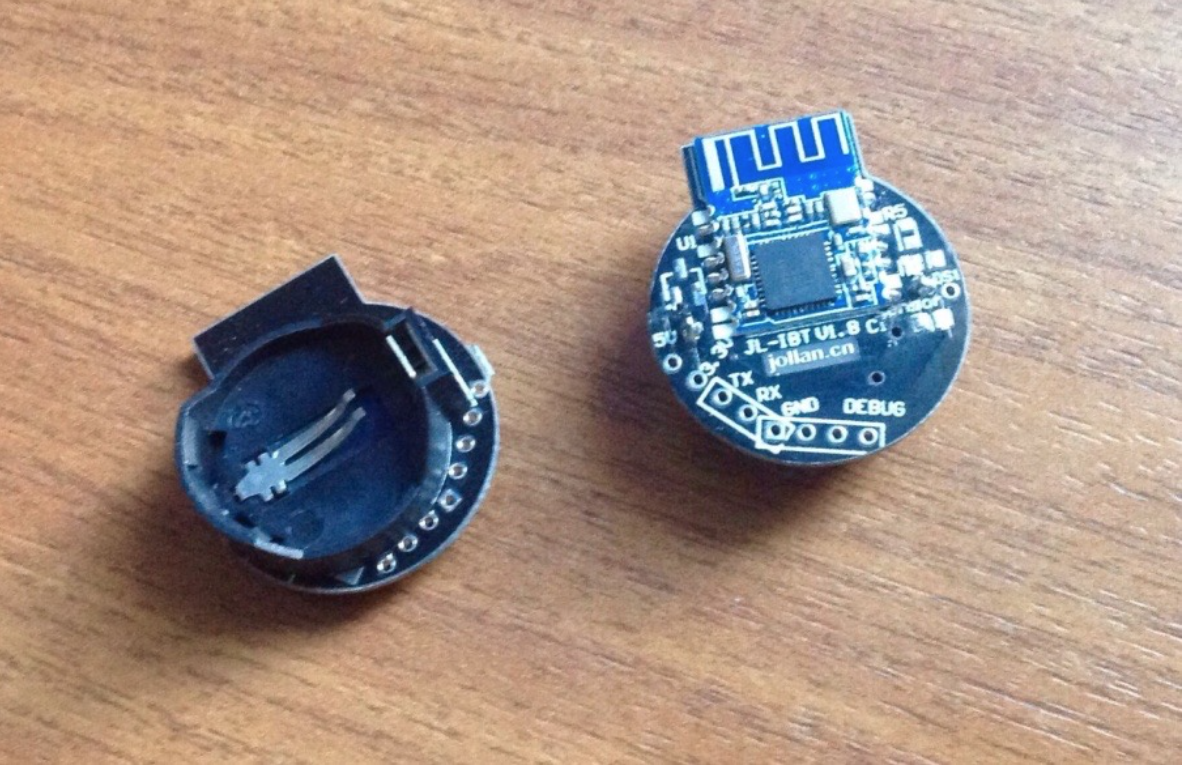
\includegraphics[scale=0.4]{img/beacons.png}
    \caption{Маячки, использованные в работе}
\end{figure}

Типичный маячок, показанный на рисунке выше, имеет довольно компактные размеры, и способен проработать всего лишь от одной батарейки до двух лет. Схемотехнически состоит из батарейки и Soc (System-On-Chip) Texas Instruments CC2540/2541 (также применяется Nordic nRF51822), представляющий собой 8051 микроконтроллер, в который загружается прошивка для реализации функции Beacon-маячка и периферийный модуль Bluetooth LE. Дальность действия маячка в среднем 10 метров (варьируется от 15-20см до 25-40м в зависимости от модели и настроек). Периодичность выдачи данных - 200мс, но это, опять же, настраивается: можно настроить и на более частую периодичность, и на более редкую. В рассматриваемой работе маячки были настроены на периодичность в 1с. Срок службы от одной батарейки в зависимости от модели - от чуть менее одного года до трёх лет (в среднем 2 года). Цена одного маячка составляет порядка 15-20 долларов. Маячок является простым устройством, который только выдаёт всем подряд в эфир свои данные (в advertising-режиме), используя Bluetooth профиль GATT (при этом к нему даже не нужно выполнять подключение), тем не менее, производители, как правило, закладывают возможность подключения к маячку с целью его удалённого конфигурирования (редактирование данных, выдаваемых в эфир, периодичность выдачи данных и мощность излучения).
    \subsection{Анализ формата входных данных}

С заданной периодичностью, циклически маячок выдает один и тот же набор данных \cite{web:HabrBig, web:HabrIOS7}:

\begin{figure}[h!]
    \centering
    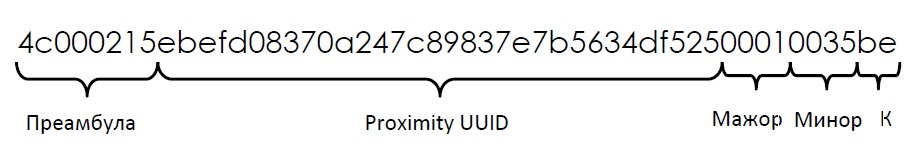
\includegraphics[width=\textwidth]{img/packageData2}
    \caption{Пример пакета, передаваемого маячком}
    \label{params}
\end{figure}

\begin{figure}[h!]
    \centering
    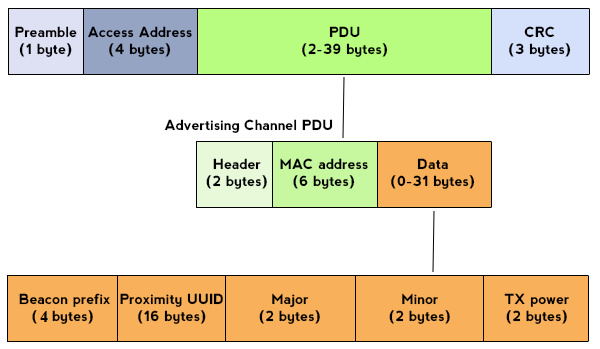
\includegraphics[width=\textwidth]{img/packageStructure}
    \caption{Общая структура Bluetooth-пакета}
\end{figure}

\textbf{Преамбула (4 байта)} - префикс пакета, позволяющий установить, что мы имеем дело именно с Beacon-маячком. Всегда равен \texttt{4c000215}. Преамбула состоит из 4-х полей: идентификатор компании (2 байта, в данном примере - \texttt{4c00}), тип (1 байт, в примере - \texttt{0x02}) и длина данных (1 байт, значение - \texttt{0x15}).

\textbf{Proximity UUID (16 байт)} – Идентификатор группы маяков. Например, если существуют несколько торговых залов, в которых требуется разместить маяки, то во всех этих залах они будут иметь один и тот же UUID, указанный при конфигурации, и это позволит отличать маяки от других, посторонних.

\textbf{Мажор (2 байта)} – позволяет различать небольшой набор маяков внутри одной группы. То есть внутри одной большой группы маяков, идентифицируемой UUID, может быть несколько подгрупп, каждая из которых идентифицируется по номеру мажора. Например, согласно приведенному выше примеру, каждому залу можно присвоить свой номер мажора. Если маяками требуется охватить несколько этажей здания - обычно с каждым этажом ассоциируют свой номер мажора.

\textbf{Минор (2 байта)} – номер, идентифицирующий сам маяк внутри мажора. Связка uuid+мажор+минор позволяет нам однозначно идентифицировать маяк и по этим данным определить координату самого маячка (обычно используется таблица соответствия маячка и его координат).

\textbf{TX Power (параметр K на рисунке выше, 2 байта)} – эталонное значение мощности маячка, представляющее собой силу сигнала на расстоянии в 1 метр от маячка и измеряется в децибелах. Измеряется это единственный раз при изготовлении маячка и вшивается в него изначально. Сравнивая эталонное значение мощности и текущее, получаемое в процессе работы, возможно вычислить расстояние до источника сигнала. Первый бит является знаковым (1 - <<$-$>>, 0 - <<$+$>>). Например, TX Power в нашем примере (см. рисунок \ref{params}, параметр <<К>>) – \texttt{0xBE}, то есть 190 в десятичной системе счисления. Тогда эталонная сила сигнала на расстоянии 1м от маячка составляет $256-190=-66$ dBm.
    \subsection{Анализ альтернативных технологий для навигации внутри помещений}

\begin{enumerate}
    \item
    \textit{RFID} – способ автоматичесткой идендификации объектов, в котором посредством радиосигналов считываются или записываются данные, хранящиеся в так называемых транспондерах, или RFID-метках. По своей функциональности, RFID, как методы сбора информации, очень близки к штрих-кодам, наиболее широко применяемым сегодня для маркировки товаров. Следовательно, RFID хорошо подойдет, например, для отслеживания посылки по большому транспортному узлу, стоит лишь снабдить весь маршрут этой посылки и ее саму RFID-метками. То есть RFID применяется там, где система знает про все. Маячки представляют собой передатчики, и мы не ориентируемся на наличие некой глобальной информации о всем состоянии, есть только информация о локальном состоянии.
    \item
    \textit{NFC} - технология беспроводной высокочастотной связи малого радиуса действия. Она предоставляет возможность обмена данными между устройствами, находящимися на расстоянии около 10 см. Вместе с существующей инфраструктурой бесконтактных карт, технология нацелена на использование в платежных системах и общественном транспорте. Надо заметить, что в своей сфере она обладает некоторыми важными преимуществами: NFC-метки потребляют мало энергии и легко встраиваются. \\ 
    Следует сделать замечание, что сам принцип работы технологий RFID и NFC не совсем подходит для решения круга задач, перечисленных ранее. На практике или их сложно встроить, ведь их требуется много (RFID), или радиус действия слишком мал, как в случае NFC.
    \item
    \textit{Навигация по Wi-Fi}. Используется уже существующая инфраструктура сетей связи – точки беспроводных сетей Wi-Fi, и это наименее затратный вариант. Методика определение координат следующая: устройство пользователя сканирует доступные Wi-Fi-точки доступа, затем информацию о них отправляет на сервер, где эти данные по базе данных сопоставляются с координатами этих точек доступа, по которым и вычисляются координаты пользователя. К сожалению, координаты Wi-Fi точек точно не известны, плюс могут меняться (перенесли Wi-Fi точку в другое место или заменили её на другую – координаты уже оказываются неверными). \\
    Точность при таком подходе оставляет желать лучшего (погрешность - до 25 метров! При использовании специально созданной Wi-Fi инфраструктуры точность достигает 3-5 метров, но это уже требует ощутимых затрат на создание и обслуживание подобной системы), да и идентицифировать клиентов по Wi-Fi, привязывая их расположение к карте помещений, проблематично: начиная с iOS 8, mac-адреса Apple-устройств (iPhone, iPad) постоянно меняются для предотвращения «рекламной» слежки.
    \item
    \textit{Геомагнитное позиционирование}. Основано на ориентировании по магнитному полю Земли и базируется на геомагнитных аномалиях как критериях для геомагнитного позиционирования (аномалии возникают вследствии неоднородности геомагнитного поля). Заключается в фиксации геомагнитных аномалий и нанесении их на карту территории, на которой предполагается ориентироваться. В дальнейшем навигация производится по составленной карте устройством, в которое встроен магнитометр. Практический пример реализации – система IndoorAtlas команды учёных из финского университета Оулу. \\
    Недостаток – высокая сложность реализации, невысокая точность. В помещениях очень много динамически меняющихся магнитных аномалий (проводка, поле в которой меняется в зависимости от подключённой нагрузки и сильно меняет конфигурацию магнитного поля вокруг себя; посетители со своими радиоэлектронными устройствами; стеллажи; тележки), сильно усложняющих навигацию, основанную на указанном способе ориентировании в пространстве.
    \item
    \textit{Системы спутниковой навигации (GPS/Глонасс и другие) + инерциальные навигационные системы (ИНС)}. Применимо, когда периодически появляется сигнал систем спутниковой навигации. Его точности по мнению современных исследователей достаточна, чтобы вычислить положение пользователя вплоть до десятка сантиметров \cite{web:GPScent}! Однако когда пользователь въезжает в тоннель, ещё доступны актуальные координаты и направление движения с GPS/Глонасс-спутников, далее в самом тоннеле сигнал теряется, и поэтому используется уже инерциальная навигационная система (ИНС, основанная на базе акселерометра, гироскопа, магнитометра), которая использует в качестве начальных условий последние актуальные данные с GPS/Глонасс до потери связи со спутником и поддерживает их актуальность на основе получаемых с датчиков данных о текущей скорости, ускорении и направлении движения до возобновления связи со спутниками. \\
    Стоит принимать во внимание, что в ИНС ошибки постоянно накапливаются, и со временем данные, полученные с ИНС, становятся все более и более отличными от действительности.
    \item
    \textit{Ориентирование по базовым станциям операторов сотовой связи (GSM)}. В зоне видимости сотового телефона/GSM-модема постоянно находятся как минимум одна базовая станция GSM, а обычно их несколько. Координаты расположения этих базовых станций известны (благодаря многочисленным навигационным сервисам (например <<Яндекс.Навигатор>>), приложение получает информацию о видимых мобильным телефоном базовых станций и текущем положении по GSM/<<Глонасс>>, и отправляет эти сведения в <<Яндекс>>, где на основе этих данных строится база соответствий <<Базовая станция-координаты>>, к которой имеется свободный доступ через предоставляемое API). Далее в модем отправляется команда "AT+CREG=2", в результате чего можно получить сообщения +CREG: с информацией о текущей подключенной базовой станции: LAC и CELLID (соответственно код зоны и идентификатор базовой станции). Отправив эти данные на один из специальных сервисов (предоставляемый <<Яндекс>>, "Google" и другими компаниями), возможно определить координаты этой базовой станции. Многие модемы позволяют получить список видимых базовых станций (БС) с указанием их LAC и CELLID - остаётся только через базы данных с координатами БС получить их координаты и методом триангуляции определить примерное местоположение пользователя. \\
    Минусы: невысокая точность (БС может быть удалена на расстоянии в 35км от пользователя, некоторые БС являются мобильными и постоянно меняют свою дислокацию).
    \item
    \textit{Использование Bluetooth-маячков iBeacon} даёт достаточную точность при приемлемом уровне финансовых затрат; перспективная технология, которая активно развивается, поэтому именно iBeacon был выбран в качестве предмета данной работы.
    \item
    \textit{Навигация, основанная на синергетическом эффекте} решает задачу определения текущего местоположения, используя все (или большинство) из перечисленных выше способов. Эффективность достигается за счёт того, что используется сразу несколько векторов определения координат, что способствует компенсации ошибок и повышению точности определения координат. На реализацию подобной системы в прошлом году фондом развития центра разработки и коммерциализации новых технологий <<Сколково>> был выделен грант в 1 млн долларов \cite{web:HabrBig}.    
\end{enumerate}
    \subsection{Анализ безопасности}

Не стоит переоценивать данную технологию и забывать о таком важном аспекте, как безопасность. На текущий момент развития трафик в процессе передачи никаким образом не шифруется, поэтому злоумышленник потенциально может провести атаку.

Выделяются 2 главных типов атак: спуффинг и пиггибэкинг \cite{web:SecuritySlides}.

\begin{itemize}
    \item
    \textit{Beacon Spoofing}. Атака основана на включении маячка или устройства, работающего как маячок, с параметрами, идентичными параметрам некоторой группы маячков. Это может быть использовано для того, чтобы симулировать некоторое событие или оповещение в месте, отличном от предполагаемого в контексте приложения. \\
    \textit{Пример угрозы:} предположим, есть некоторый магазин, использующий маячки для приветствия новых посетителей. Злоумышленник копирует настройки маячков, и впоследствие это позволяет ему разослать приветственное уведомление пользователям, которые находятся в абсолютно другой локации. Это может спровоцировать недоумение и, в конечном итоге, неудовлетворенность программным продуктом.
    \item
    \textit{Beacon Piggybacking, или Hijacking}. Атака основана на применении уже существующих маячков, предназначенных для некоторого приложения, в своем, стороннем приложении. Это может быть использовано для получении аналитики, основанной на оригинальный маячках, а также в рассылке сообщений и симуляции событий, не относящихся к предполагаемым. \\
    \textit{Пример угрозы:} пусть кофейня «А» конкурирует с кофейней «Б». «А» начинает использовать приложение с использованием маячков. В ответ кофейня «Б» разрабатывает свое приложение с информацией об идентификаторах чужих маячков. В результате каждый раз, как пользователь с установленным приложением от кофейни «Б» заходит в кофейню «А», на его устройство приходит оповещение о скидках на кофе в «Б».
\end{itemize}

Неприятный инцидент произошел на выставке потребительской электронике (Consumer Electronics Show – CES) в 2014 году. Для всех желающих была организована «охота за сокровищами», в рамках которой через приложение пользователи должны были определить место, где якобы зарыт сундук с кладом. Однако еще до начала мероприятия неизвестная группа хакеров взяла apk-файл приложения, проанализировала его структуру через декомпилятор, и смогла извлечь параметры всех используемых маячков. Это давало всю необходимую информацию, и победить таким способом можно было даже не выходя из дома \cite{web:ScavengeHunt}.

Выделяют 4 способа защиты:

\begin{itemize}
    \item
    \textbf{Геолокационная проверка}. После получения оповещения от одного из новых (в рамках текущей сессии) маячков, устройство использует геолокационный сервис, чтобы убедиться, что маячок физически действительно находится поблизости.
    \item
    \textbf{Идентификация на основе начального значения (seed)}. Используются маячки с периодически меняющимся UUID. Алгоритм смены, в свою очередь, основан на некотором цифровом значении, хранимом отдельно. Через единый SDK происходит обновление, идентификация и синхронизация всего процесса. Маячок, не прошедший проверку – потенциальный вредитель – будет выкинут из рассмотрения.
    \item
    \textbf{Облачное подтверждение}. Способ базируется на основе предыдущего, но роль связующего звена на себя берет облачный сервис, а не локальный SDK. 
Этот механизм уже используется в маячках компании Estimote, и известен под названием “UUID Rotation”. Секретный ключ, определяющий смену идентификаторов, хранится на облачной платформе Estimote Cloud.
    \item
    \textbf{Управление на уровне аппаратных средств}. Начальные параметры и их возможное обновление берут на себя аппаратные средства – контроллеры. При этом оповещение об обновлении приходит от облачного сервиса отдельно на контроллеры и отдельно на устройство пользователя. После этого контроллеры обновляют UUID маяков. В дальнейшем проверка маячков будет происходить на устройстве без использования сервиса.
\end{itemize}

Преимущества и недостатки перечисленных методов представлены в таблицах 1 и 2, соответственно.

\begin{sidewaystable}
    \caption[Caption]{Достоинства различных способов защиты.}
	\begin{tabu} to \textheight { | X[l] | X[l] | X[l] | X[l] | X[l] | }
	\hline
	\textit{Способ защиты} & 
	    \textbf{Геолокационная проверка} & 
	    \textbf{Идентификация на основе генерации случайных чисел} &
	    \textbf{Облачное подтверждение} &
	    \textbf{Управление на уровне аппаратных средств} \\
	\hline
	
	\textit{Преимущества} & 
	    1. Наиболее дешевый способ \newline 
	    2. Простой в конфигурации и поддержке \newline
	    3. Может быть легко включен или выключен в любой момент \newline
	    4. Позволяет использовать традиционный iBeacon-формат для лучшей совместимости & 
	    
	    1. Позволяет защититься от перечисленных типов атак \newline
	    2. Нет привязки к геолокации или Интернет-соединению \newline
	    3. Не требует дополнительного оборудования &
	    
	    1. Позволяет в большей степени защититься от перечисленнных способов атак \newline
	    2. Не требуется подключение дополнительных устройств \newline
	    3. Усложняет процедуру проведения атаки для злоумышленника &
	    
	    1. Надежный уровень защиты \newline
	    2. Предоставляет устройство для обновления и обслуживания маячков \newline
	    3. Изменения легко применить к существующей системе \newline
	    4. Позволяет использовать традиционный iBeacon-формат для лучшей совместимости \\
	\hline
	\end{tabu}
\end{sidewaystable}

\begin{sidewaystable}
\caption[Caption]{Недостатки различных способов защиты.}
\begin{tabu} to \textheight { | X[l] | X[l] | X[l] | X[l] | X[l] | }
\hline
\textit{Способ защиты} & 
    \textbf{Геолокационная проверка} & 
    \textbf{Идентификация на основе генерации случайных чисел} &
    \textbf{Облачное подтверждение} &
    \textbf{Управление на уровне аппаратных средств} \\
\hline

\textit{Недостатки} & 
    1. Не защищает против piggybacking-атак \newline
    2. Геолокационная относительность не дает такой же точности, как остальные методы \newline
    3. Определение локации может являться причиной задержки в начале сессии &
    
    1. Сложен в модификации в случае неполадок \newline
    2. UUID маячков могут быть легко определены злоумышленником \newline
    3. Более сложное развертывание \newline
    4. Формат использования не поддерживается в приложениях Apple &
    
    1. Сложен в модификации в случае неполадок \newline
    2. Сложен в развертывании \newline
    3. Задержки в использовании могут отразиться на удобстве использовании приложения \newline
    4. Предполагает наличие Интернет-соединения \newline
    5. Формат использования не поддерживается в приложениях Apple &
    
    1. Наиболее дорогой тип размещения \newline
    2. Требует наличия дополнительного набора устройств \newline
    3. Не работает для маячков, расположенных на удалении от остальных \newline
    4. Предполагает наличие Интернет-соединения (периодически)\\
 \hline
\end{tabu}
\end{sidewaystable}

\clearpage
\newpage

Примечательно, что Apple iOS SDK на уровне реализации не позволяет приложению сканировать эфир на обнаружение BLE-пакетов. Обязательным условием является явная конфигурация UUID, major и minor-идентификато\-ров \cite{web:CoreBlRestrict}.

    \subsection{Выбор языка и технологий программирования}

\textbf{Objective-C} - компилируемый объектно-ориентированный язык программирования, используемый корпорацией Apple, построенный на основе языка Си и парадигм Smalltalk. В частности, объектная модель построена в стиле Smalltalk — то есть объектам посылаются сообщения.

Язык Objective-C является надмножеством языка C, поэтому C-код полностью понятен компилятору Objective-C.

Компилятор Objective-C входит в GCC и доступен на большинстве основных платформ. Язык используется в первую очередь для Mac OS X (Cocoa) и GNUstep — реализаций объектно-ориентированного интерфейса OpenStep. Также язык используется для iOS (Cocoa Touch).

\textbf{Swift} - мультипарадигменный объектно-ориентированный язык программирования, созданный компанией Apple для разработчиков iOS и OS X. Swift работает с библиотеками Cocoa и Cocoa Touch и совместим с основной кодовой базой Apple, написанной на Objective-C. Swift задумывался как более безопасный язык в сравнении с Objective-C. Язык поддерживается в среде программирования Xcode; программы на нем компилируются при помощи Apple LLVM и используют рантайм Objective-C, что делает возможным использование обоих языков (а также чистого С и С++) в рамках одной программы.

Для реализации библиотеки был выбран язык Objective-C, так как язык хорошо поддерживается стандартной IDE “XCode”, отлично документирован и обладает широким сообществом программистов. Кроме того, в Objective-C лучшая по сравнению со Swift поддержка вставок кода на C, а именно на нем написаны алгоритмы трилатерации, рассматриваемые в данной работе.
    \subsection{Анализ предоставляемого API}

Для indoor-навигации Apple предоставляет библиотеку CoreLocation. Она содержит несколько основных сущностей, использованных в работе:

\begin{itemize}
    \item
    \texttt{CLBeacon}. Класс, инкапсулирующий как идентификаторы маяка (uuid, major, minor), так и информацию, используемую при ранжировании (rssi, accuracy, proximity).
    \item
    \texttt{CLBeaconRegion}. Класс, содержащий идендификаторы группы маяков (uuid, [major, [minor]]). С его помощью можно удобно разделять группы маячков, находящихся, например, на разных этажах, и работать с каждой группой по отдельности.
    \item
    \texttt{CLLocationManager}. Центральный класс API, который может отслеживать маячки в указанном регионе (\texttt{CLBeaconRegion}), рассылая событиями как факты входа или выхода в зону действия маячков (\textit{mo\-ni\-to\-ring}), так и прием пакетов для определения расстояния до источника (\textit{rang\-ing}).
\end{itemize}

Таким образом, Apple представила не только формат на BLE-маячки iBeacon, ставший уже широко распространенным, но и удобные средста для работы с ними.
    \subsection{Анализ лиейного фильтра Калмана}

В рамках исследуемой работы возникает небходимость фильтровать некоторые данные. Прежде всего, к ним относятся значения RSSI, получаемые от маячков.

Фильтр Калмана был выбран на основании нескольких положений \cite{eikhoff}:

\begin{enumerate}
    \item
    Фильтр имеет рекуррентную форму, благодаря чему он удобен для программирования. Кроме того, так как новые оценки формируются на основе старых, нет необходимости хранить весь массив наблюдений, что экономит память и время работы.
    \item
    Алгоритм фильтрации одновременно представляет собой непосредственное описание способа реализации фильтра.
    \item    
    Его легко распространить на нестационарные сигналы; это относится и к случаю, когда наблюдения начинаются в произвольный момент времени.
    \item
    Легко распространяется на многомерный случай.
\end{enumerate}

К тому же, скользящее среднее при большем размере окна (обозачим размер за $N$) будет отражать не актуальные данные, а лишь усреднение за последние $N$ измерений. Калман же при большем доверии новому значению больше приближает показание к последнему измеренному, при этом не исключая корректировки выбросов.

Фильтр Калмана использует динамическую модель системы (например, физический закон движения), известные управляющие воздействия и множество последовательных измерений для формирования оптимальной оценки состояния. Алгоритм состоит из двух повторяющихся фаз: \textit{предсказание} и \textit{корректировка}. 

На первом рассчитывается предсказание состояния в следующий момент времени (с учетом неточности их измерения). На втором новая информация с датчика корректирует предсказанное значение (также с учетом неточности и зашумленности этой информации). Важно отметить, что задача фильтрации – получить наиболее близкое значение к реальной величине.

Рассмотрим алгоритм фильтра в общем случае для следующих имеющихся данных: 

\begin{numcases}{}
    x_{k+1} = x_k + u_k + \xi_k \label{new_x}
    \\ 
    z_k = x_k + \eta_k \label{new_z}
\end{numcases}
где $x_k$ – измеряемая величина; \\
$u_k$ – член, отвечающий за контроль системы извне (закон, по которому изменяется величина $x$); \\
$\xi_k$ – ошибка модели, то есть разница между реальным значением и рассчитанным;\\
$\eta_k$ – ошибка, образовавшаяся в результате измерения сенсором;\\
$z_k$ – полученные данные с сенсора;\\
$x_{k+1}$ – новое значение величины на очередном шаге итерации.

Задача состоит в том, что, зная неверные показания сенсора $z_k$, найти хорошее приближение для истинного значения $x_k$. Это хорошее приближение мы будем обозначать как $x_k^{opt}$.

Будем рассуждать по индукции. Представим, что мы уже нашли отфильтрованное значение с сенсора $x_k^{opt}$. Можно предположить, что на шаге $k+1$ система эволюционирует согласно закону \ref{new_x}, и сенсор покажет значение, близкое к $x_k^{opt} + u_k$. С другой стороны, зная соотношение \ref{new_z}, мы будем знать неточное значение сенсора $z_{k+1}$.

Идея Калмана состоит в том, что чтобы получить наилучшее приближение к истинной координате $x_{k+1}$, мы должны выбрать золотую середину между показанием неточного сенсора и $x_k^{opt} + u_k$ — нашим предсказанием того, что мы ожидали от него увидеть. Показанию сенсора мы дадим вес $K$ а на предсказанное значение останется вес $(1-K)$:
\[
    x_{k+1}^{opt} = Kz_{k+1} + (1-K)(x_k^{opt} + u_k)
\]
Коэффициент K называют коэффициентом Калмана.

Согласно выводам самого Калмана, коэффициент имеет свойство стабилизироваться после небольшого числа итераций \cite{kalmanKinect}.

Алгоритм обладает достаточной гибкостью: он позволяет задать априорную информацию о характере системы, связи переменных, и на основании этого строить более точную оценку. Кроме того, даже в случае отсутствия априорной информации фильтр дает отличные результаты \cite{web:habrKalmanTut, web:habrKalmanIntro}.
    \subsection{Анализ оптимального расположения маячков в помещении}

Мы имеем начальную систему уравнений, основанную на методе трилатерации:
\[
\begin{cases}
    (x_0-x_1)^2+(y_0-y_1)^2=r_1^2 \\
    (x_0-x_2)^2+(y_0-y_2)^2=r_2^2 \\
    (x_0-x_3)^2+(y_0-y_3)^2=r_3^2 \\
\end{cases}
\]

Однако данная система не может дать однозначного решения в виде точки, если, например, общая область пересечения кругов не является точкой. Назовем в таком случае область такого общего пересечения областью ошибки локализации. Введем также обозначение: пусть величина ошибки варьируется в интервале $(-\epsilon, \epsilon)$. Используя это, определим:
\[
C_{p_i}=
    \{ 
        (x; y) \in R^2 | (x-x_i)^2+(y-y_i)^2 \leq (r_i+\epsilon_i)^2, \\
                                             (x-x_i)^2+(y-y_i)^2 \geq (r_i-\epsilon_i)^2 
    \}
\]

В приведенном выше определении можно заметить, что $\epsilon_i=0, \cap_i C_{p_i}$ образует единственную точку. В случае, когда $\epsilon_i>0, \cap_i C_{p_i}$ образует область с площадью, отличной от нуля.

В исследовании \cite{han2009reference} математически доказано, что данная площадь будет минимальна (учитывая, что величина $\epsilon$ мала), если маячки установлены симметрично. То есть в случае трилатерации оптимальным вариантом будет расположение их в узлах равностороннего треугольника, а дальнейшая установка новых устройств для покрытия большей площади будет выполнена, как на рисунке \ref{optimum_placement}.

\begin{figure}[ht]
    \centering
    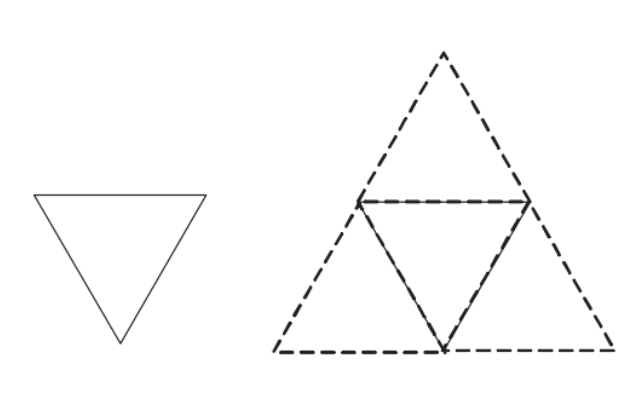
\includegraphics[scale=0.6]{img/triangles}
    \caption{Оптимальное расположение маячков}
    \label{optimum_placement}
\end{figure}

Расположение в узлах квадратов дает несколько худший результат (ошибка в среднем больше на 5,3\%), а случайное расположение маячков увеличивает ошибку на 34,9\% \cite{bulusu2001adaptive}.

    \subsection{Анализ задачи выбора оптимального набора маячков}

Существует целое семейство алгоритмов, называемое “OASIS” – Opti\-mum Anchor Selection algorIthmS, что в переводе и значит «выбор оптимального набора маячков». Для работы с GPS существует функционал, называемый $GDOP$ – Geometric Dilution Of Precision, то есть <<геометрическое ослабление точности>>. Данная величина отражает, насколько на текущий момент взятое созвездие спутников вляет на результирующую точность.

Вычислить GDOP возможно по следующей формуле:
\begin{equation} \label{for:gdop}
    GDOP(M, \phi)=\sqrt{ \frac{M}{\sum_i\sum_{j,j>i}|\sin(\phi_{ij})|^2} }
\end{equation}
где $M$ – количество спутников, рассматриваемых в рамках нахождения текущей локации, а $\phi$ – угол между каждой из пар спутников. При этом чтобы вычислить $GDOP$ для отдельно взятой точки, необходимо знать ее положение. В приложениях, использующих GPS, начальное грубое вычисление исходной позиции может быть допущено ввиду больших дистанций между пользователем и спутниками. В рамках задачи определения локации внутри помещений такой подход неприемлем и не может быть использован без каких-либо изменений.

Рассмотрим альтернативные методы OASIS:
\begin{itemize}
    \item
    \textbf{Совместная кластеризация}. Подход метода заключается в выборе $k$ лучших по силе сигнала (RSSI) маячка для дальнейшего вычисления координат.
    \item
    \textbf{Простая выпуклая оболочка}. В данном методе рассматриваются дистанции, определенные при анализе величины сигнала от каждого из маячков $n_1, n_2, ..., n_N$. Фунционал выпуклой оболочки, обозначаемый С, может быть вычислен по формуле:
    \[
        C \equiv \{ \sum_{j=1}^N \lambda_j n_j : \lambda_j \geq 0 \}, \sum_{j=1}^N \lambda_j = 1
    \]
    \item
    \textbf{Сила сигнала}. Используемая в данной работе техника, заклю\-чаю\-щая\-ся в выборе трех маячков с наиболее сильным сигналом вне зависимости от их расположения.
    \item
    \textbf{Выбор, основанный на определении площади}. Согласно исследованию, проведенному М.Миронововой и Х.Халвисом \cite{mironovova2011calculation}, большая площадь, сформированная тремя спутниками, образует лучшее (то есть меньшее) значение $GDOP$. Применяя это к поставленной задаче, мы перебираем все возможные треугольники, образованные тройками маячков, выбирая наибольший по площади из них.
    \item
    \textbf{Периметр}. Метод достаточно схож по своей сути с приведенным выше, но при рассмотрении треугольника учитывается его периметр. Периметр также показывает линейную независимость координат образовавших его маячков. С другой стороны, использование периметра бесполезно в рамках некоторых сценариев (например, нахождение трех маячков на одной прямой).
    \item
    \textbf{Плотность}. Алгоритм, рассматривая все комбинации маячков, вычисляет все возможные координаты пользователя. После этого область с наибольшей плотностью возможных координат пользователя выбирается в качестве результата, а конечной точкой обычно берется центроид промежуточных результатов.
    \item
    \textbf{Мультилатерация}. Если рассматривать сразу $N$ маячков, то возможно составить систему уравнений для вычисления положения пользователя, учитывая показания каждого из них. \\
    Положим, что координата узла $i$ есть $b_i$. Необходимо вычислить положение пользователя $p$. Показания маячков равны $d_i$, соответственно. В идеальной ситуации мы имеем:
    \[
        || b_i - p ||^2_2=d_i^2
    \]
    Перепишем левую часть в виде
    \begin{equation} \label{for:neededPos}
            || b ||^2_2 + || p ||^2_2 - 2b_i^Tp = d_i^2    
    \end{equation}
    Учитывая, что всего участвуют в расмотрении $M$ маячков, снова возможно переписать выражение в следующем виде для вычисления позиции пользователя:
    \begin{equation} \label{for:p}
        p = 0.5B^+(a+\gamma)    
    \end{equation}
    при этом мы воспользовались заменой $\gamma = || p ||^2_2$ и $[a]_i = || b ||^2_2 - d_i^2$, а также вектор-столбец $B = [p_1, p_2, ..., p_M]^T$. Нотация $B^+$ означает псевдообращение Мура-Пенроуза. Чтобы решить \ref{for:p}, необходимо вычислить $\gamma$:
    \[
        \gamma = p^T p = [0.5B^+(a+\gamma)]^T [0.5B^+(a+\gamma)]
    \]
    В нашем случае мы выбираем $\gamma$, которая бы давала наименьшую среднюю ошибку между каждым из значений $p1, p2, ..., p_M$ и искомой позицией (см. \ref{for:neededPos}). \\
\end{itemize}

    В работе \cite{artemenko2012comparison}, показано, что в рамках проводимого ряда экспериментов, наименьшая средняя ошибка достигается при использовании методов, основанных на выборе по силе сигнала, совместной кластеризации и мультилатерации. 
    
    Важно отметить, что те методы, которые не использовали RSSI-по\-ка\-за\-тель сигнала явно (как например основанные на площади или периметре), давали худшие результаты. 
    
    Наконец, при увеличении вовлеченных в процесс вычисления маячков, разные подходы адаптировались лучше или хуже. Так, мультилатерация, несмотря на свою точность, значительно замедлялась в работе из-за решения сверхдетерминированной системы уравнений. 
    
    Руководствуясь вышеприведенными рассуждениями, был выбран метод, основанный на использовании трех маячков с наилучшими сигнал-шу\-мо\-вы\-ми показателями.
    \subsection{Реализация алгоритма, основанного на сравнении локационных отпечатков}

Локационные «отпечатки пальцев» – набор признаков, присвоенных некоторой заведомо известной точке пространства \cite{elbes2013precise}.  В рамках задачи будем считать, что этим набором признаком является вектор из эталонных показателей RSSI, принятых от каждого из маячков.

Смысл алгоритма тогда будет состоять в следующем: пользователь в некоторый момент времени определяет ряд значений RSSI. Этот набор сравнивается с остальными с целью нахождения ближайшего «отпечатка», значения которого отличается минимально в рамках принятой метрики. И так как положение каждого из «отпечатка» заранее известно, становится возможным определить положение пользователя.

Данную задачу можно рассматривать как задачу классификации. Так, каждый отпечаток $FP_i$ в точке пространства $i \quad (i=\overline{1,N})$ может быть представлен как $FP_i = \{ RSSI_1^{FP_i}, RSSI_2^{FP_i}, ..., RSSI_M^{FP_i} \}$, и соответствующая ему локация есть $L_i^{FP} = (X_i, Y_i)$.

Если представить положение пользователя как $T$, то ему сопоставим отпечаток $ S = \{ RSSI_1^T, RSSI_2^T, ..., RSSI_M^T \}$. После этого возможно найти дистанцию между $S$ и $FP_i$:
\begin{equation} \label{for:D}
    D^T_{FP_i} = \sqrt{ \sum_{j=1}^N ( RSSI_j^{FP_i} - RSSI_j^T )^2 }
\end{equation}

Будем считать $M$ количеством маячков, участвующих в рассмотрении. Теперь на основе расстояния можем вычислить вероятность того, что объект $Т$ находится около отпечатка $FP_i$ с измерениями $S$:
\begin{equation} \label{for:Prob}
    P(FP_i | S) = \frac{1}{ D^T_{FP_i} }
\end{equation}

Тогда правило определения локации можно сформулировать так: \textit{искомая точка – $i$ – если $P(FP_i | S) > P(FP_j | S)$, где $i,j = \overline{1,N}$. Ей соответствует локация $L_i^{FP}$.}

В реальности искомая позиция пользователя не является дискретной, и поэтому возникает необходимость интерполяции. Эта процедура осуществляется с помощью следующего преобразования, представленного ниже:
\[
    LT(x,y) = \sum_{i=1}^N P(FP_i | S) L_i^{FP}(x,y)
\]
, где $(x,y)$ - координаты $FP$.

В работе \cite{elbes2013precise} предложено дополнение для данного подхода, называемое Budgeted Dynamic Exclusion (BDE, "бюджетное динамическое исключение"). Суть модификации сводится к следующему: сравниваются показания $j$ и отпечаток $i$. Если некоторая пара значений RSSI, соответствующих одному и тому же маяку, меньше установленной константы, именуемой бюджетом, то эти два значения выкидываются из вектора с остальными значениями RSSI. Это приводит к тому, что оцениваемое формулой \ref{for:D} Евклидово расстояние уменьшается, и, соответственно, степень доверия, вычисляемая с помощью формулы \ref{for:Prob}, увеличивается.

Главным препятствием в работе такой системы является дифракция, отражение и рассеяние сигнала, принимаемого от маяков \cite{liu2007survey}. Кроме того, возникают сложности, связанные с выходом из строя маячков. Ведь в таком случае необходимо либо переснимать показания сигнал-шума от оставшихся маячков заново, либо предусмотреть дополнительную логику в приложении и работе алгоритма в целом. Оба способа достаточно затратны по времени.

Хотя данный метод нахождения пользовательской локации был использован, например, на конференции GeekPicnic, проведенного в Москве в 2015г. \cite{web:habrGeekPicknic}, в итоговую версию библиотеки, разработанной в рамках данной работы, алгоритм не включен.    \clearpage \newpage
\section{Реализация}

 
    \subsection{Основные классы библиотеки}

\subsubsection{BeaconLocation}

Класс \texttt{BeaconLocation} – центральный класс библиотеки. Предполагается, что пользователь начинает работу с инстанцирования этого класса. Во время создания \texttt{BeaconLocation} создает необходимые объекты \texttt{CoreLoca\-tion} (\texttt{CLBeaconRegion}, \texttt{CLLocationManager}), а так же подписывается на обновления данных, получаемых от маячков.

Кроме того, здесь же происходит создание классов \texttt{Processor}, который ответственен за вычисление новых координат пользователя, и \texttt{Floor}, который является хранилищем всех идендификаторов маячков, их координат и очередных показаний.

\subsubsection{Floor}

Класс \texttt{Floor} инкапсулирует маячки, расположенные на этаже. Также пре\-до\-став\-ляет набор методов, с помощью которых пользователь может добавить новые маячки, получить информацию об уже имеющихся и удалить указанные. Предполагается, что задающие их координаты измеряются в метрах, так как обновления значений расстояний до маячков тоже формируются в метрах самой библиотекой \texttt{CoreLocation}.

\subsubsection{Processor}

Класс \texttt{Processor} - ядро библиотеки. По умолчанию он подписывается на события об изменении вычисленных расстояний до маячков, и вычисляет на их основе новое положение пользователя. 
Пользователю предлагаются 3 готовых алгоритма, а также делегат, с помощью которого он может реализовать и использовать собственный метод. Кроме того, есть возможность использовать комбинацию из имеющихся алгоритмов для достижения лучшего результата.

Степень доверия результату каждого из алгоритмов может быть указана в параметрах метода \\
\begin{small}
\texttt{-(void)setAlgorithmsAndTrusts:(NSDictionary<NSNumber*, NSNumber*>*)algorithms}
\end{small}

Переданные в паре с каждым из алгоритмов числа нормируются к единице. Пусть первый алгоритм вычислил положение пользователя как точку с координатами $(1; 1)$. Второй используемый алгоритм - как точку $(5; 5)$. По умолчанию, все алгоритмы эквивалентно важны, и общим результатом будет среднее арифметическое: точка $(3; 3)$. Если второй алгоритм вдвое более важен, чем первый, то результат будет вычислен как $0,66*(5; 5) + 0,33*(1; 1)$, то есть $(3,66; 3,66)$.

\subsubsection{Attractor и Spot}

Для того, чтобы сделать приложение более отзывчивым во время приближения пользователя к некоторому объекту, в библиотеке предусмотрены классы \texttt{Attractor} и \texttt{Spot}. 

\texttt{Spot} - класс, представляющий некоторую <<горячую точку>> в локационном контексте приложения, другими словами, место, в котором мы ожидаем увидеть пользователя чаще, чем в другом (витрина в магазине, экспонат в музее). 

Работа с ними осуществляется через класс \texttt{Attractor}. После того, как точки добавлены, а положение пользователя вычислено, \texttt{Attractor} приближает положение пользователя к ближайшей <<горячей точке>>, основываясь на определенным пользователем коэффициенте (<<сила притяжения>> - \texttt{attractorPo\-wer}). Учтена и <<мертвая зона>>, внутри которой \texttt{Attractor } перестает приближать положение пользователя к указанной отметке.

Все это позволяет создавать более дружественный интерфейс разрабатываемого приложения.
    \subsection{Реализация алгоритма трилатерации, основанного на определении силового центра}

Другим вариантом реализации метода трилатерации может быть алгоритм, предложенный бельгийскими исследователями В.Пьерло, М.Ур\-бин-Шоф\-фреем и М.Ван Другенброек, которые свели проблему к решению системы линейных уравнений \cite{pierlot2011new}.

Чтобы объяснить суть метода, прежде всего, необходимо ввести понятие о так называемом \textit{силовом центре} (“power center” или “radial center”) трех окружностей – уникальной точке, обладающей равной мощностью (“power”) по отношению к этим окружностям. Мощность $P$ точки при этом может быть найдена по формуле:
\begin{equation} \label{for:power}
    P_{c,p} = (x-x_c)^2 + (y-y_c)^2 - R^2
\end{equation}
где ${x, y}$ – координаты точки, для которой вычисляется мощность, ${x_c, y_c}$ – координаты центра окружности радиуса $R$. Согласно формуле \ref{for:power}, если точка лежит на окружности, мощность равна нулю; меньше нуля в случае, когда точка находится внутри окружности и больше нуля, когда находится вне окружности.

\textit{Силовой линией }(“power line”) двух окружностей назовем такое геометрическое место точек, обладающих равной мощностью по отношению к этим окружностям. 

Она перпендикулярна прямой, соединяющей центры данных окружностей и проходит через область их взаимного пересечения (в случае наличия такового). Если рассматриваются три окружности, такие, что никакие две из них не расположены в одной точке, и центры которых не коллинеарны, то для них можно определить силовой центр – точкой пересечения силовых линий. На приведенном ниже рисунке силовой центр обозначен точкой.

\begin{figure}[ht]
    \centering
    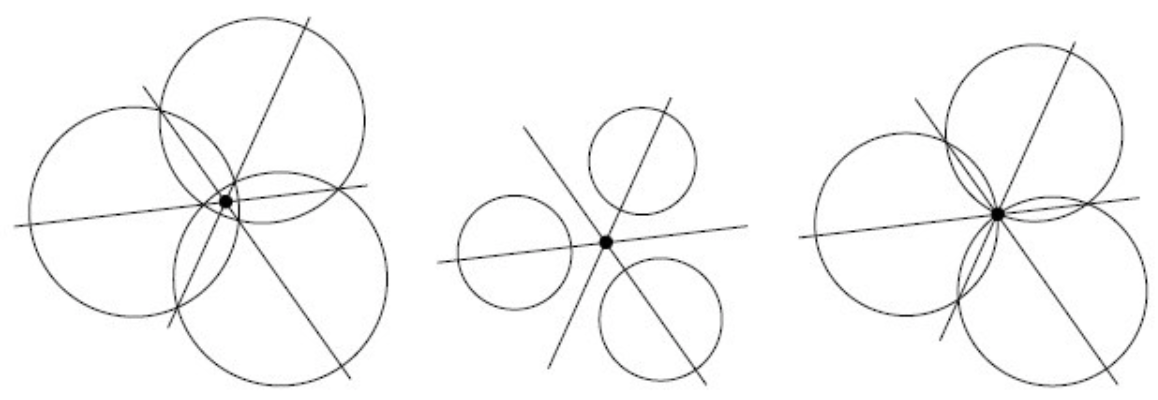
\includegraphics[width=\textwidth]{img/powerCenters}
    \caption{Определение силового центра для окружностей различных радиусов}
\end{figure}

Нахождение координаты точки пересечения двух прямых – задача, имеющая линейную сложность. В данном случае мы можем, учитывая формулу~\ref{for:power}, просто приравнять мощности.
\begin{align}
    (x-x_1)^2 + (y-y_1)^2 - R_1^2 &= (x-x_2)^2 + (y-y_2)^2 - R_2^2 \notag \\
    \Rightarrow x(x_1-x_2) + y(y_1-y_2) &= \frac{x_1^2+y_1^2-R_1^2}{2} - \frac{x_2^2+y_2^2-R_2^2}{2} \notag \\
    \Rightarrow x(x_1-x_2)+y(y_1-y_2) &= k_1 - k_2 \notag
\end{align}

Введен дополнительный коэффициент $k$, равный мощности источника относительно некоторой окружности, деленный на два:
\[
    k_n = \frac{x_n^2+y_n^2-R_n^2}{2}
\]

Наконец, чтобы определить координаты точки пересечения силовых линий, достаточно решить систему линейных уравнений:

\begin{numcases}{}
    x(x_1-x_2) + y(y_1-y_2) = k_1-k_2 \notag
    \\
    x(x_2-x_3) + y(y_2-y_3) = k_2-k_3 \label{for:system}
    \\
    x(x_3-x_1) + y(y_3-y_1) = k_3-k_1 \notag
\end{numcases}

Можно заметить, что одно из уравнений в системе может быть получено путем сложения двух других, что является, в свою очередь, доказательством пересечения трех силовых линий лишь в одной точке. Ее точные координаты можно определить по следующим формулам:
\[
    x_r = \frac{ 
	    \begin{vmatrix}
	    k_1-k_2 & y_1-y_2 \\
	    k_2-k_3 & y_2-y_3
	    \end{vmatrix}}{D},  \quad
    y_r = \frac{
    \begin{vmatrix}
   	    x_1-x_2 & k_1-k_2 \\
	    x_2-x_3 & k_2-k_3
    \end{vmatrix}}{D} 
\]

\[
    D = \begin{vmatrix}
	    x_1-x_2 & y_1-y_2 \\
	    x_2-x_3 & y_2-y_3
    \end{vmatrix} = \begin{vmatrix}
        x1 & y1 & 1 \\
        x2 & y2 & 1 \\
        x3 & y3 & 1
    \end{vmatrix}
\]

Определитель матрицы $D \neq 0$, если центры окружностей не коллинеарны, тогда же, соответственно, существует решение приведенной системы уравнений \ref{for:system}. В противном случае найти координаты пересечения прямых в явном виде нельзя.

\begin{figure}[ht]
    \centering
    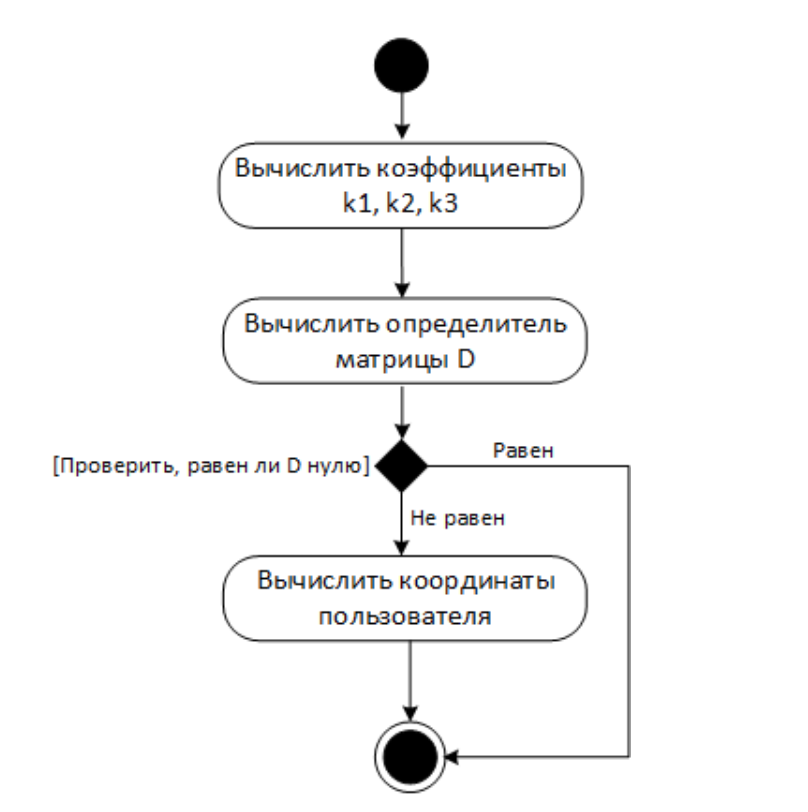
\includegraphics[scale=0.5]{img/powerCenterActivity}
    \caption{Activity-диаграмма рассматриваемого алгоритма}
\end{figure}

Исходный код, реализующий данный метод, приведен в приложении 1.
    \subsection{Реализация алгоритма трилатерации, основанном на пересечении сфер}

В геометрии трёхмерная проблема трилатерации представляет собой нахождение координат точки пересечения трёх сфер, которые определяются путём решения системы уравнений. Чтобы упростить вычисления, полагаем, что центры всех трех сфер лежат в плоскости $z=0$, один из них совпадает с началом координат, второй — лежит на оси $x$. Наложенные ограничения не уменьшают общности: к такому виду может быть приведена любая система соответствующих уравнений путем перехода к другой системе координат. Чтобы найти решение в исходной системе координат, к решению, найденному в этой (приведенной) системе координат, применяются преобразования, обратные к тем, которые позволили исходное множество из трех точек привести в соответствие с ограничениями.

С первого взляда может показаться, что задача определения координаты устройства по нескольким маячкам схожа с задачей, которая решается спутниками GPS, и, соответственно, мы тоже должны решать задачу о пересечении сфер. К тому же, маяки могут быть закреплены в помещении на разных высотах. Но на практике этим можно пренебречь, отбросив $z$-координату. Предпосылкой для этого является и то, что хотя маячки могут находиться на различной высоте, на одной и той же высоте находится пользователь. Таким образом, задача сводится к работе с окружностями.

\begin{figure}
    \centering
    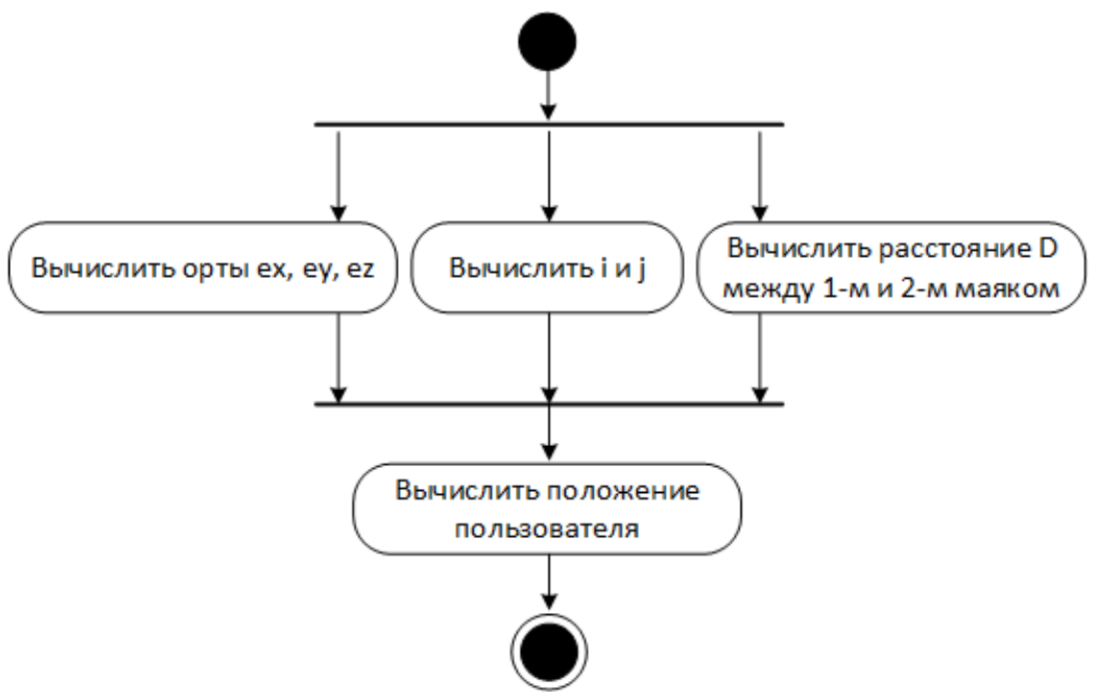
\includegraphics[scale=0.5]{img/sphereIntAct}
    \caption{Activity-диаграмма алгоритма пересечения сфер}
\end{figure}    
    \subsection{Реализация адаптивного геометрического алгоритма}

Прежде всего, следует объяяснить принцип работы геометрического алгоритма.

Геометрический алгоритм опирается на взаимоположение окружностей и их радиусы, и результирующие точки пересечения имеют ключевое значение. На рисунке \ref{fig:scenarios} показаны наиболее часто возникающие сценарии (точки, соответствующие пересечениям окружностей, обозначены как $a, b, c,$ и так далее). 

\begin{figure}[h]
    \centering
    \begin{subfigure}[h]{0.4\textwidth}
        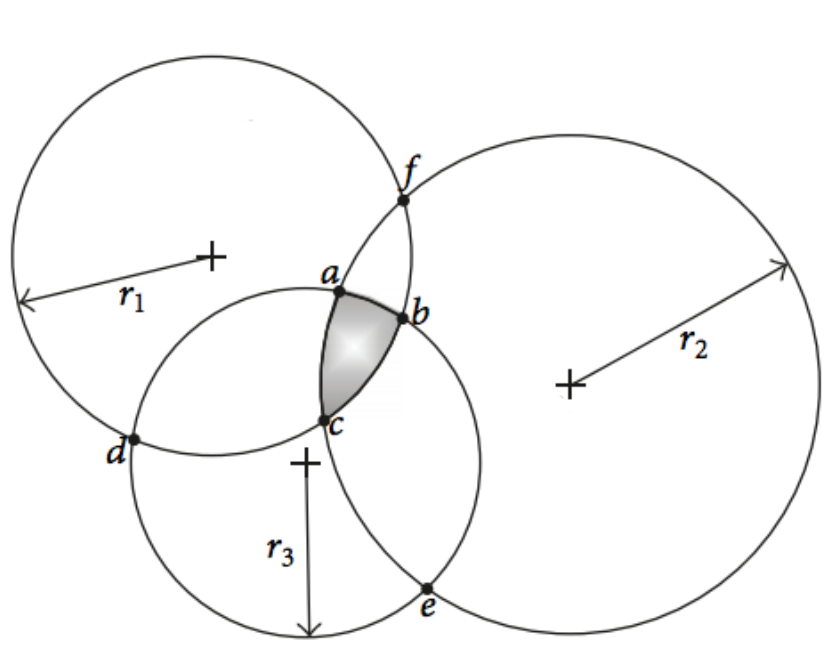
\includegraphics[width=\textwidth]{img/circlesInter}
        \caption{}
        \label{fig:inter}
    \end{subfigure}
    \begin{subfigure}[h]{0.4\textwidth}
        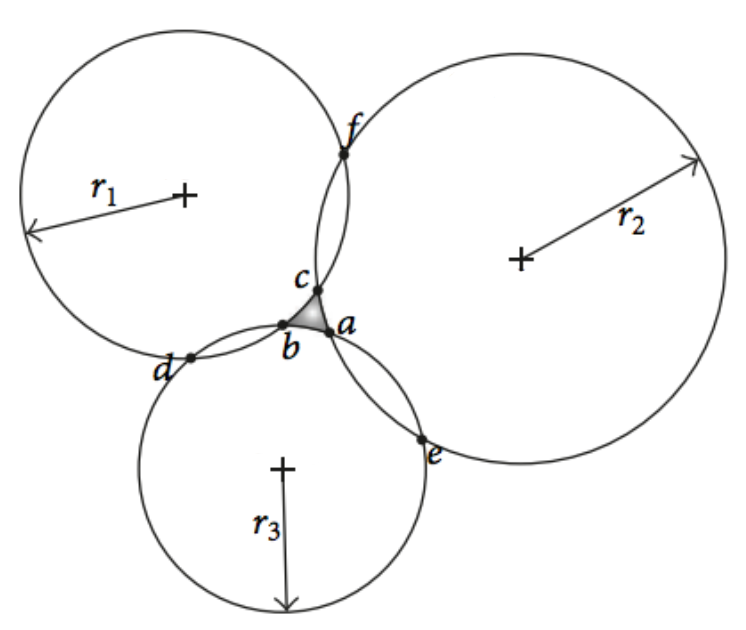
\includegraphics[width=\textwidth]{img/circlesOuter}
        \caption{}
        \label{fig:outer}
    \end{subfigure}
    \caption{Наиболее часто встречающиеся сценарии при работе геометрического алгоритма}
    \label{fig:scenarios}
\end{figure}

В случае, изображенном на рисунке \ref{fig:inter}, нас интересуют только три точки из шести, так как они формируют область, принадлежащую всем трем окружностям.

На рисунке \ref{fig:outer} более сложный сценарий, ведь общей области пересечения всех трех окружностей нет. Следовательно, мы должны воспользоваться другой логикой для нахождения искомой области. Конкретнее, для каждй пары точек, образовавшейся в результате пересечения пары окружностей, нас удовлетворяет та точка, которая находится ближе к третьей окружности (например, из точек $a$ и $e$ будет выбрана $a$, так как она находится ближе к окружности с радиусом $r_1$).

Наконец, искомым положением пользователя является центроид, вычислимый по формуле \ref{for:centroid}.
 
\begin{equation} \label{for:centroid}
    x = \frac{1}{K}\sum^K_{l=1}x_l, \quad y = \frac{1}{K}\sum^K_{l=1}y_l, \quad  l = 1,2,...,K
\end{equation}

$K$ в представленной выше формуле означает количество подходящих точек пересечений. Для случая с тремя окружностями $K=3$.

В работе \cite{brida2013novel} представлена идея \textit{адаптивного геометрического алгоритма}. В сущности, геометрический алгоритм, описанный выше, является частным случаем, а точнее - первой итерацией адаптивного геометрического алгоритма. 

\begin{figure}[ht]
    \centering
    \includegraphics[width=\textwidth]{img/agaDiag}
    \caption{Блок-схема, представляющая функционирование адаптивного геометрического алгоритма}
    \label{fig:aga}
\end{figure}

Благодаря данной первой итерации получен набор точек пересечения. Суть алгоритма сводится к пропорциональному увеличению или уменьшению всех трех радиусов окружностей так, чтобы общая область пересечений (см. случай на рисунке \ref{fig:inter}) была наименьшей. Конечный этап - нахождение положения пользователя - осуществляется по формуле \ref{for:centroid}. Алгоритм работы проиллюстрирован на рисунке \ref{fig:aga}.

В настоящей работе предложена модификация алгоритма для увеличения скорости его работы. Суть изменения сводится к следующему: для случая, показанного на рисунке \ref{fig:inter}, вместо пропорционального уменьшения радиусов, вычисляются координаты центроида точек пересечения. Для случая, показанного на рисунке \ref{fig:outer}, алгоритм функционирует, как описано выше. 

Полный листинг конечной версии алгоритма представлен в приложении В.
    
\clearpage \newpage
   
\renewcommand{\bibname}{Список литературы}
\addcontentsline{toc}{section}{\bibname}

\bibliographystyle{gost71s}
\bibliography{references}{}

\end{document}